\section{Gabor filters}
In this section, we will implement 2D detection using a Gabor filter. We will first play with two toy examples in 1D and 2D to understand the fundamentals, then we will attempt to have your computer play the game of ``Where's Waldo''.


\begin{enumerate}
\item \textbf{Gabor filter in 1D}

  In this question we will consider the script \verb!gabor1d_script.m! in the homework kit: it generates a 1D signal of increasing frequency \verb!s! as well as a vector \verb!s_w! containing ground-truth frequencies (see figure \ref{incr_freq}).
  \begin{figure}[ht!]
    \begin{center}
      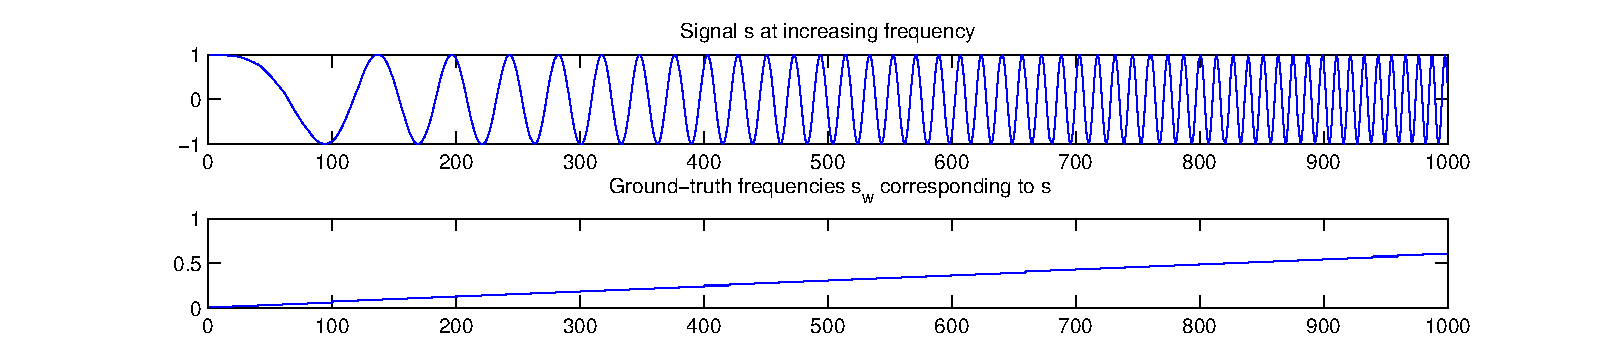
\includegraphics[width = \textwidth]{images/incr_freq_signal.pdf}
    \end{center}
    \caption{\label{incr_freq} Signal at increasing frequencies and corresponding ground-truth frequencies.}
  \end{figure}

  \begin{enumerate}
  \item \points{1} Complete the function \verb!gaussian1d.m! that returns discrete normalized centered Gaussian of given standard deviation $\sigma$ and length.
  \item \points{2} Complete the function \verb!gaborFilter1D.m! that returns a pair of Gabor quadrature filters at given spatial period \verb!T_f! in pixels, Gaussian envelope $\sigma$ and length. The two filters correspond respectively to the real and imaginary part of the Gabor filter we defined in class.
  \item \points{4} Complete the script \verb!gabor1d_script.m! to compute the filter response: \verb!r1!, \verb!r2! are the imaginary and real parts of the response, and \verb!energy! is the magnitude of the response (complex norm).
  \item \points{2} Using the script, plot figures for two distinct values of $T_f$ and check that the maximum response matches the ground truth.
  \end{enumerate}

\item \textbf{Gabor filter in 2D}

  We now consider the same problem in 2D: we want to detect patterns with a specific spatial period \emph{and} orientation in the image represented in figure \ref{incr_freq_2d}.
    \begin{figure}[ht!]
    \begin{center}
      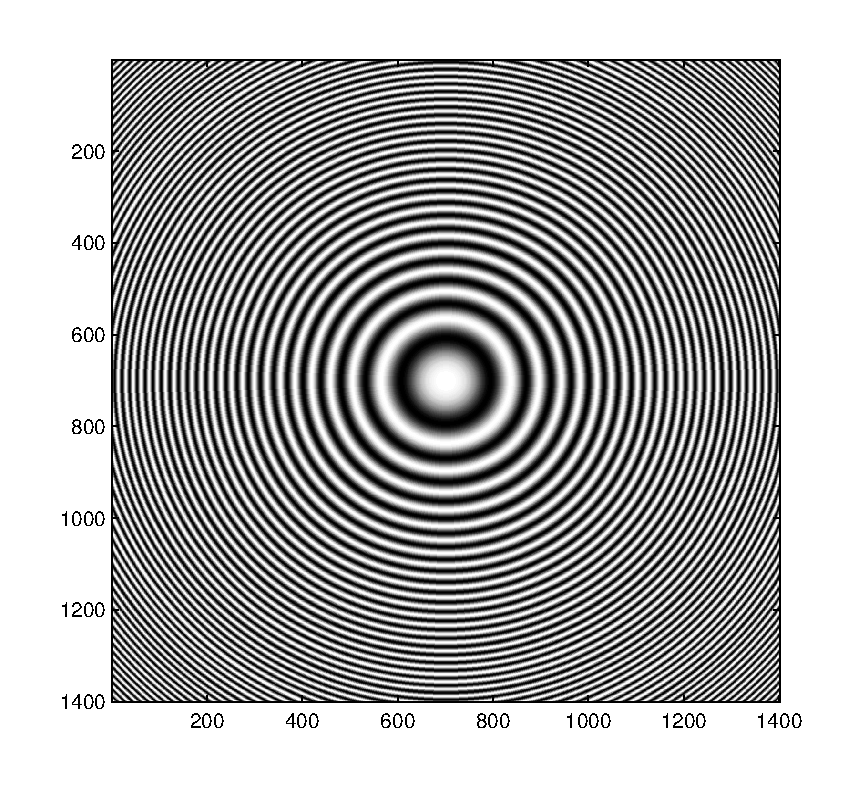
\includegraphics[width = 0.5\textwidth]{images/incr_freq_2d.pdf}
    \end{center}
    \caption{\label{incr_freq_2d} Image containing a range of frequencies and orientations.}
  \end{figure}

  \begin{enumerate}
  \item \points{2} Complete the function \verb!gaussian2d.m! that returns discrete normalized centered 2D Gaussian of given covariance matrix $\Sigma$ and size.
  \item \points{5} Complete the function \verb!gaborFilter2D.m! that returns a pair of Gabor quadrature filters to detect a given spatial period \verb!T_f! in pixels \textbf{and} orientation \verb!theta! in degrees. The two filters correspond respectively to the real and imaginary part of the Gabor filter we defined in class. 
  \item \points{4} Complete the script \verb!gabor2d_script.m! to compute the filter response: \verb!r1!, \verb!r2! are the imaginary and real parts of the response, and \verb!energy! is the magnitude of the response (complex norm).
  \item \points{2} Using the script, plot figures for two distinct values of $T_f$ and check that the maximum response matches the ground truth.
  \end{enumerate}

\item \textbf{Where's Waldo?}

  Now we consider the classical game of finding Waldo (a character with a red-and-white striped shirt) in an image like figure \ref{im:waldo}. We are going to use the function \verb!gaborFilter2D! to craft a filter for horizontal oscillation at an appropriate frequency.
  \begin{figure}[ht!]
    \begin{center}
      
\includegraphics[width = 0.5\textwidth]{images/waldo.jpg}
    \end{center}
    \caption{\label{im:waldo} Where's Waldo?}
  \end{figure}
  
  \begin{enumerate}
  \item \points{2} Read through the script \verb!waldo_script.m! and describe what it does in a couple sentences.
  \item \points{2} Look at the first plot (run the script up to line 28 included) and explain in a few words the formula for \verb!im_red!, line 14.
  \item \points{6} Complete the function \verb!determineStripePeriod.m! that interactively determines the spatial frequency of Waldo-like stripes in the image: you only need to complete the part computing \verb!T_y! after the user clicks on a peak of the fft.
  \item \points{8} Complete end of the script \verb!waldo_script.m! to compute the response of the Gabor filter and the detection mask: figure \ref{waldo_example} shows a part of the image multiplied by \verb!detection_mask!, which is a double matrix equal to $1$ in the candidate areas and $0$ anywhere else.

    You can compute \verb!detection_mask! by thresholding \verb!energy! and by applying \verb!imdilate! with a \verb!'disk'! structuring element of size $30$, to make the zones slightly bigger and include a small portion of the image around the detected stripes: it makes it more convenient to see Waldo's head! Read the documentation of \verb!imdilate! and \verb!strel! for more details.
    \begin{figure}[ht!]
      \begin{center}
        \includegraphics[width = 0.5\textwidth]{images/waldo_example_output.png}
      \end{center}
      \caption{\label{waldo_example} Example output: the energy response is thresholded and dilated, and the resulting detection mask is applied to the image to show only candidate zones with stripes at the right frequency. }
    \end{figure}
  \end{enumerate}
\end{enumerate}



%%% Local Variables: 
%%% mode: latex
%%% TeX-master: "../hw3"
%%% End: 
